\documentclass{beamer}


\usetheme[progressbar=frametitle]{metropolis}
\setbeamertemplate{frame numbering}[fraction]
\useoutertheme{metropolis}
\useinnertheme{metropolis}
\usefonttheme{metropolis}
\usecolortheme{spruce}
\setbeamercolor{background canvas}{bg=white}

\definecolor{mygreen}{rgb}{.125,.5,.25}
%\usecolortheme{crane}
\usecolortheme[named=mygreen]{structure}
\title{Graph Nueral Network}
\subtitle{Temporal and Spatial Air Polution Measurement Station}
\author{Phiphat Chomchit}
\institute{CMU}

\date{}
\begin{document}
% Fill color in block
\metroset{block=fill}
	\begin{frame}
		\titlepage
	\end{frame}

	\begin{frame}[t]{What is Graph Neural Network?}\vspace{10pt}
	 
		\begin{block}{Graph definition}
			A graph $\mathcal{G}$ is defined as a tuple of a set of nodes/vertices $V$, and a set of edges /links $E$: $\mathcal{G}=(V,E)$. Each edge is a pair of two vertices, and represents a connection between them. 
		\end{block}
		For instance, let's look at the following graph:
		\begin{figure}
			\centering
			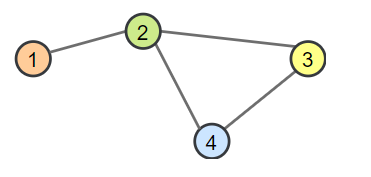
\includegraphics[scale=0.5]{sg.png}
		\end{figure}
	
	The vertices are $V=\{1,2,3,4\}$,\\ and edges $E=\{(1,2), (2,3), (2,4), (3,4)\}$.
	\end{frame}
	
	\begin{frame}[t]{What is Graph Neural Network?}\vspace{4pt}
		\begin{block}{Definition of Adjacency Matrix}
			\vspace{0.5em}
			The \textbf{adjacency matrix} $A$ is a square matrix whose elements indicate whether pairs of vertices are adjacent, i.e. connected, or not. In the simplest case, $A_{ij}$ is 1 if there is a connection from node $i$ to $j$, and otherwise 0.
			\vspace{0.5em}
		\end{block}
		
		$$
		A = \begin{bmatrix}
		0 & 1 & 0 & 0\\
		1 & 0 & 1 & 1\\
		0 & 1 & 0 & 1\\
		0 & 1 & 1 & 0
		\end{bmatrix}
		$$
		
		keep in mind that $A$ is a symmetric matrix ($A_{ij}=A_{ji}$)
	\end{frame}
	
	\begin{frame}[t]{Graph Convolutions}\vspace{4pt}
		\begin{enumerate}
			\item GCNs are similar to convolutions in images in the sense that the "filter" parameters are typically shared over all locations in the graph. 
			\item At the same time, GCNs rely on message passing methods, which means that vertices exchange information with the neighbors, and send "messages" to each other.
		\end{enumerate}
		
		\begin{figure}
			\centering
			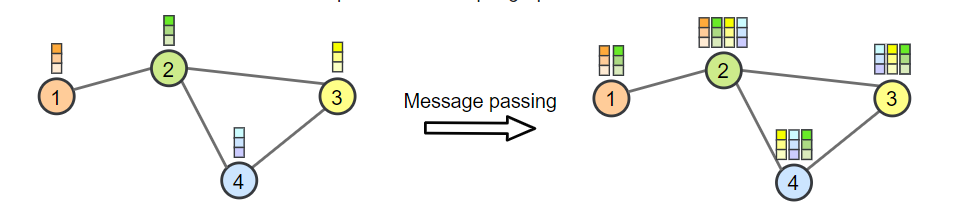
\includegraphics[scale=0.4]{sg2.png}
		\end{figure}
	\end{frame}
	
	\begin{frame}[t]{Graph Convolutions}\vspace{4pt}
		 Given the previous features of nodes $H^{(l)}$, the GCN layer is defined as follows:
		
		$$H^{(l+1)} = \sigma\left(\hat{D}^{-1/2}\hat{A}\hat{D}^{-1/2}H^{(l)}W^{(l)}\right)$$
		\begin{enumerate}
			\item $W^{(l)}$ is the weight parameters with which we transform the input features into messages ($H^{(l)}W^{(l)}$). 
			\item To the adjacency matrix $A$ we add the identity matrix so that each node sends its own message also to itself: $\hat{A}=A+I$. 
			\item $\hat{D}$ which is a diagonal matrix with $D_{ii}$ denoting the number of neighbors node $i$ has. 
			\item $\sigma$ represents an arbitrary activation function.
	\end{enumerate}
	\end{frame}

	\begin{frame}[t]{Structured Sequence Modeling with Graph Convolutional\\ Recurrent Networks}
		GCRN model modeling and predicting time-varying graph-based data. The core idea is to merge CNN for graph-structured data and RNN to identify simultaneously meaningful spatial structures and dynamic patterns. A generic illustration of the proposed GCRN architecture is given by.
		\begin{figure}
			\centering
			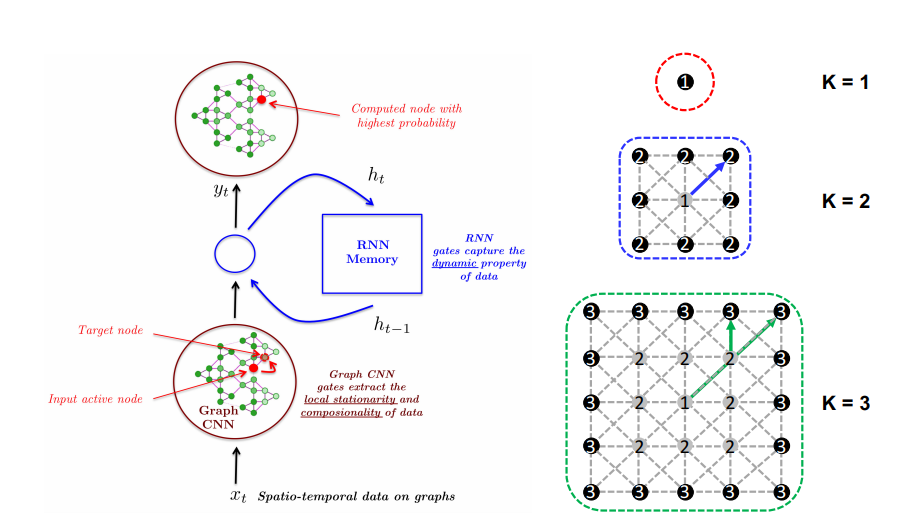
\includegraphics[scale=0.3]{tgcn.png}
		\end{figure}
	\end{frame}
	
	\begin{frame}{Structured Sequence Modeling with Graph Convolutional\\ Recurrent Networks}
		\begin{figure}
			\centering
			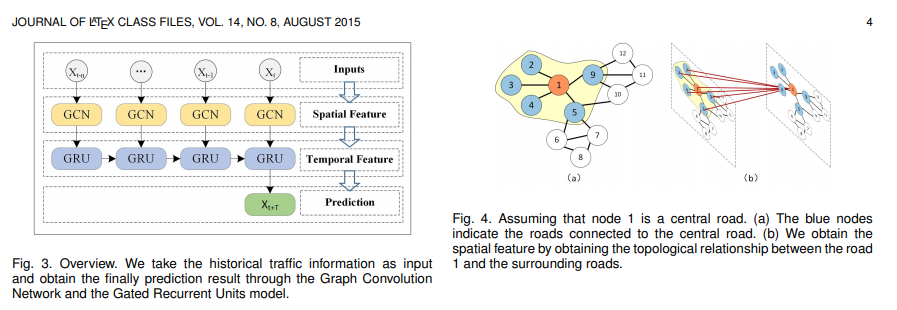
\includegraphics[scale=0.5]{tgcn2.png}
		\end{figure}
	\end{frame}

	\begin{frame}[t]{PM2.5 datasets}
		\begin{figure}
			\centering
			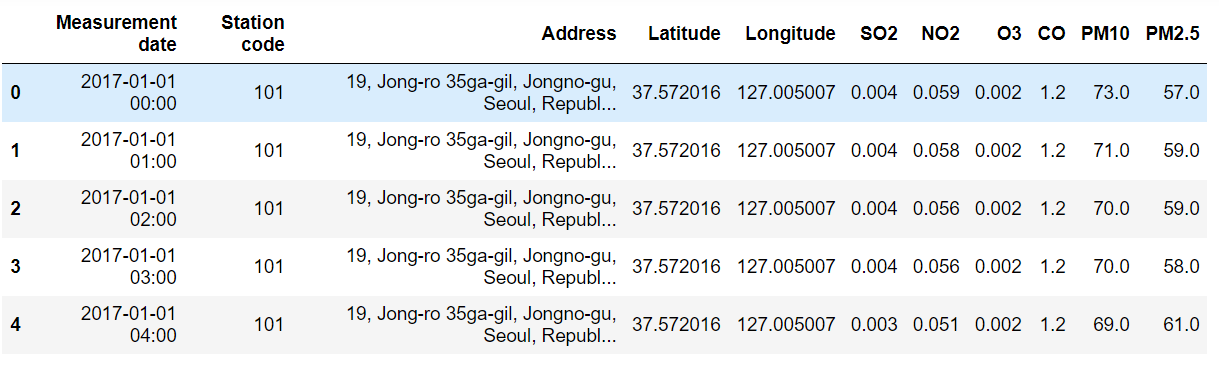
\includegraphics[scale=0.3]{df.png}
			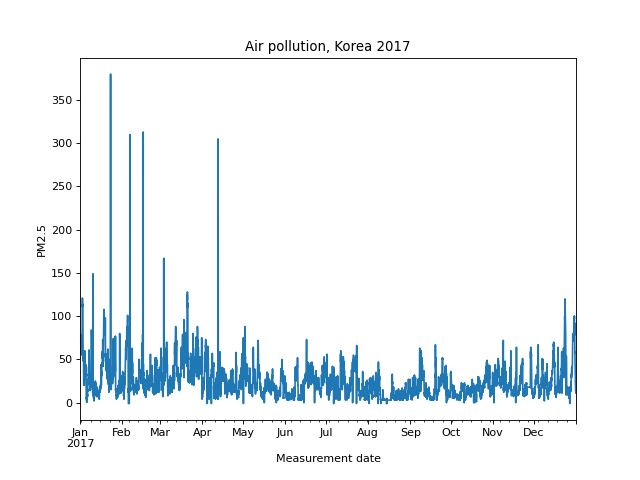
\includegraphics[scale=0.3]{pm25.png}
		\end{figure}
	\end{frame}

	\begin{frame}{Stations}
		\begin{figure}
				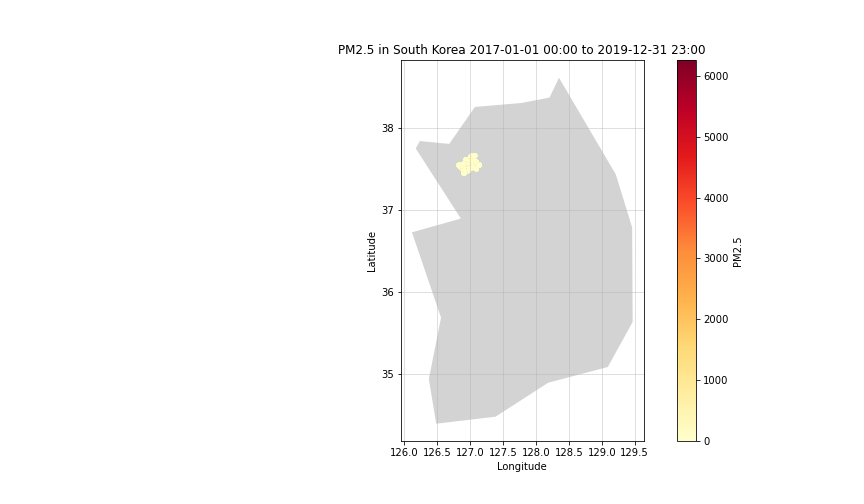
\includegraphics[scale=0.2]{korea_station.png}
				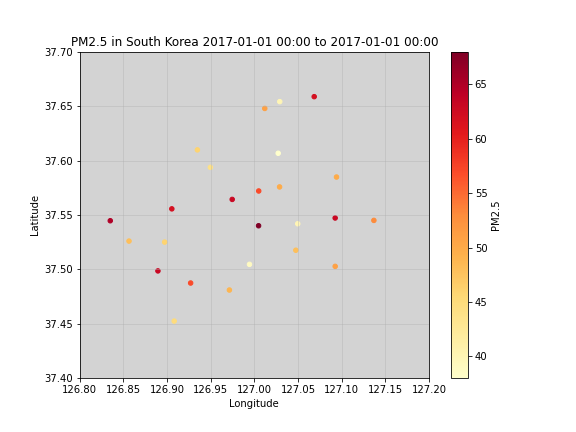
\includegraphics[scale=0.22]{station_pm.png}
		\end{figure}
	\end{frame}

	\begin{frame}{Stations}
		\begin{figure}
			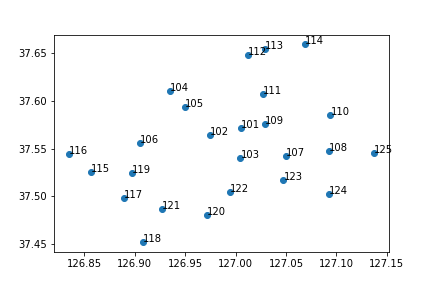
\includegraphics[scale=0.5]{station_code.png}
		\end{figure}
	\end{frame}

	\begin{frame}{Any Quation?}
		\begin{figure}
			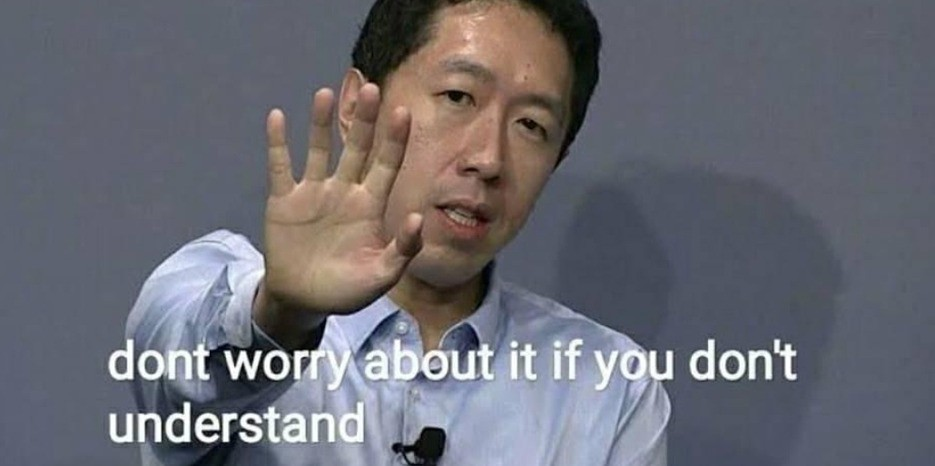
\includegraphics[scale=0.3]{ng.jpg}
		\end{figure}
	\end{frame}
	\begin{frame}[standout]
		Thnk you!
	\end{frame}
\end{document}